\chapter{Evaluation and Results}
In this chapter the EVS bridge is evaluated for performance and function. The chapter describes the modes of deployment used for evaluation and the baselines used for measurement and comparison. Wherever eligible a brief discussion of the result is provided with necessary parameters. 


\section{Evaluation Environment}
In Table 5.1, the components working together to form the evaluation environment are listed. At the core of the set up is an Open vSwitch built from the tree with release tag 2.6.1 accelerated by Intel Data Plane Development Kit built from the source with release tag 16.11.2. The hypervisor support comes from Linux-KVM with QEMU 2.9.0 for emulation, running on an Intel(R) Xeon x86_64 CPU with 16 cores. The operating system used is Ubunutu xenial 16.04.2 LTS running a 4.4.0.79-generic kernel. 
\begin{center}
	\captionof{table}{Evaluation Environment} \label{tab:title} 
	\begin{tabular}{ |c|c| } 
		\hline
		Processor &  Intel(R) Xeon(R) CPU E5-2630 v3 @ 2.40GHz  \\
		\hline 
		Architecture &  x86_64  \\ 
		\hline
		CPU(s) & 16  \\ 
		\hline
		Kernel & 4.4.0.79-generic \\
		\hline
		Distribution & Ubuntu xenial 16.04.2 LTS \\
		\hline
		Open vSwitch & 2.6.1 \\
		\hline
		Intel DPDK & 16.11.2 \\
		\hline
		Qemu & Qemu Emulator 2.9.0 \\
		\hline
		Ryu & 4.0 \\
		\hline		
	\end{tabular}
\end{center}

\section{System under Test}
The system under test during the evaluation is the Event Processing enabled Open vSwitch(EVS) bridge. Firstly the performance of the EVS bridge is measured in terms of link bandwitdh and average round trip time and compared with that of a standard OVS bridge. This is important because an addition of functionality to the OVS bridge should not result in a performace degradation that will make the OVS bridge unusable for the generic switching scenarios it was originally designed for. 
\newline
Secondly, the EVS bridge is evaluated with respect to the problem statement - described in Chapter 1.2 - that there is a performance gain to be attained when aspects of event processing are offloaded on to the underlying network. To evaluate the performance, an  application(evntsrc) is implemented to generate events, and another application(evntsink) is developed to consume the packets and measure latency. Standard packet generators cannot be used for evaluation because of the need to control the format of the packet payload. Performance of the EVS bridge is compared against a custom light-weight userspace application(evntbroker) emulating an event processing engine. The evntbroker application bridged on the standard OVS. The flow-path of data in the two systems is captured in figure 5.1. We can see that EVS bridge replaces the udpbroker and reduces the number of packets in the system. Although the evntbroker does not preform the role of full-fledged complex event processing engine, it is sufficient to provide a baseline for the event processing operations built in to the EVS bridge. The point-to-point latency between evntsrc and evntsink is measured in both the systems- under two deployment scenarios - and the results discussed.

 \begin{figure}[H]    
	\caption{Data Flow in EVS vs OVS}
		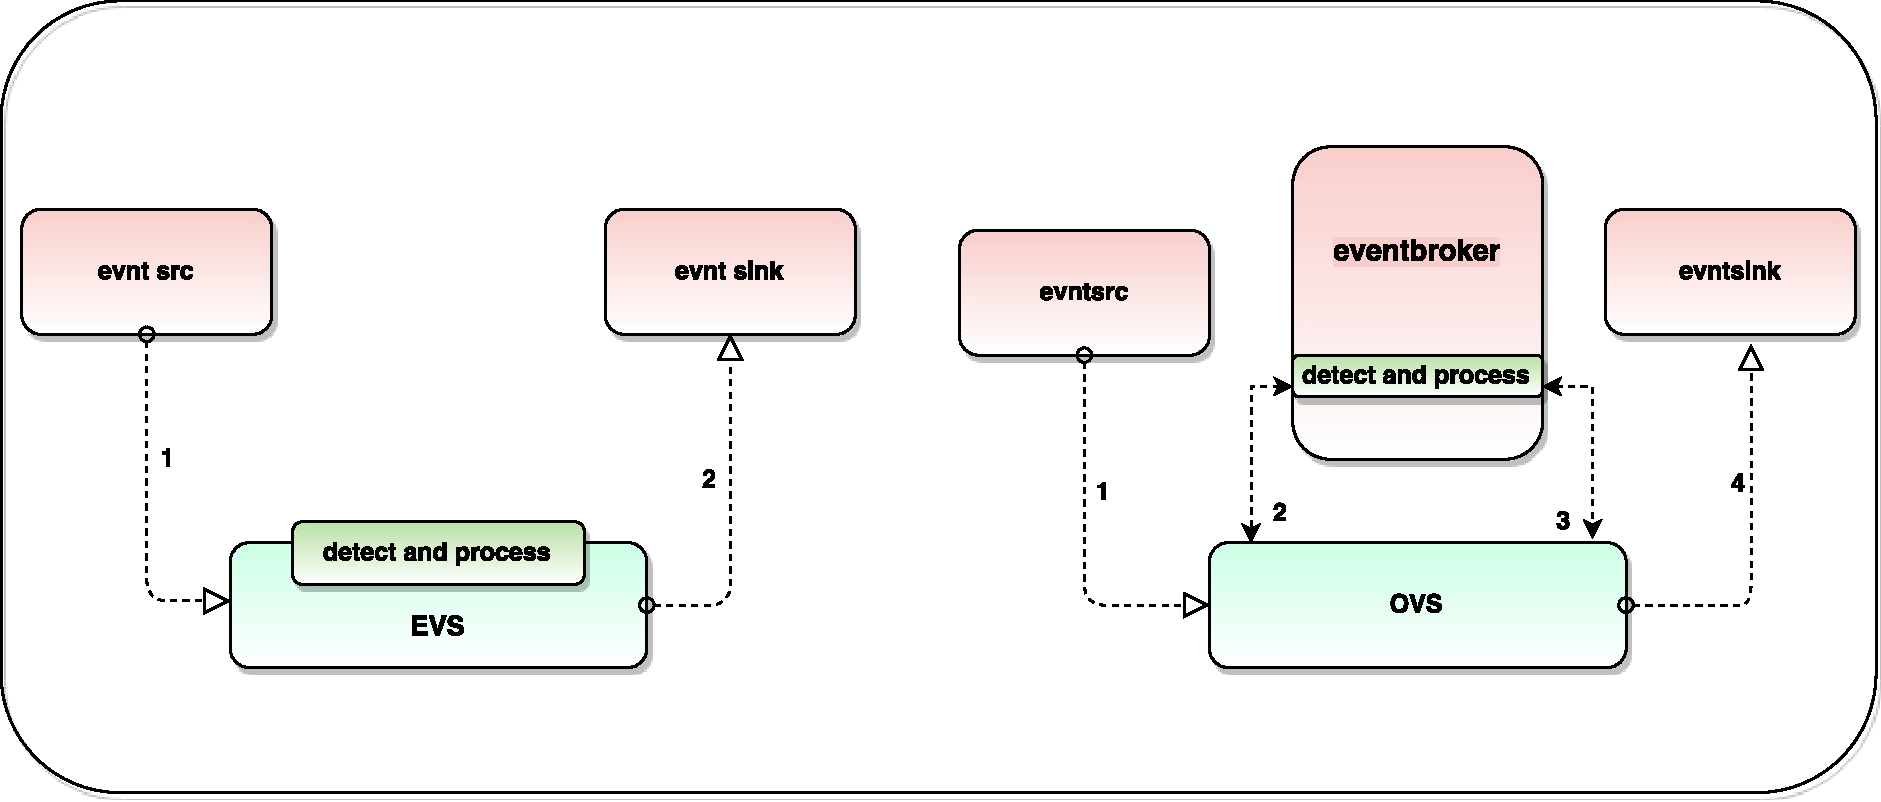
\includegraphics[height=7cm]{evsovs.pdf}
\end{figure}



Thirdly, we measure the performance of the EVS bridge for the following additional parameters:
\begin{itemize}
	\item Measure of latency with increasing size of event types.
	\item Measure of latency with increasing number of event types.
	\item Measure of latency with increasing percentage of filtered flows.
	\item Measure of latency with increasing number of matched event attributes. 
	\item Measure of latency with event attributes detection and redirection.
	\item Measure of latency with compare operations performed on event attributes.
\end{itemize}

The Evaluation is performed in two deployment modes:
\begin{itemize}
	\item Network Namespaces: As discussed in Chapter 3.7, a network namespace is a logically separate network stack within the same host machine. Since each namespace has its own network stack and can be attached with virtual Ethernet or physical ports, they offer a perfect development environment for Open vSwitch. During the evaluation phase, namespaces were bridged on Open vSwitch using TAP devices. The set-up, methodology and results are discussed in detail in section 5.4
	\item Qemu-KVM Guests: As discussed in Chapter 3.8, Qemu-KVM provide a combination of device emulation and virtual machine monitoring to set up guest virtual machines in a physical host. The evaluation set up involves Open vSwitch accelerated by Intel DPDK as a hypervisor switch bridging QEMU-KVM guests. The set-up, methodology and results are discussed in detail in section 5.5.
\end{itemize}


\section{Apparatus for Evaluation}
As briefly discussed in the previous chapter 5.2 and illustrated in figure 5.1, the three components needed for the evaluation are:
\begin{itemize}
	\item Event Source: The EVS bridge implementation handles events only if the packets have a custom tag in the packet. All other packets without the tag are sent through the standard processing flow. Once the tag is detected, the EVS bridge parses the packet payload to derive the event types and event attributes. Hence the packets have to follow the  format \textit{[tag,event_type,event_attribute1,event_attribute2]}. To this end, a Java based Event Source generator, \textit{evntsrc}, has been implemented to generate UDP packets in the established format.
		
	\item Event Sink: The events are consumed by an event sink which is responsible for measuring the point to point latency from source to sink. The \textit{evntsink} application has been implemented to consume events and measure the latency.
	
	\item Event Broker: A custom event broker, \textit{evntbroker}, is implemented to perform the operations built-in to the EVS bridge. The evntbroker provides an alternate flow-path for events to that of the flow-path in the EVS bridge. And the flow-path of data is similar to that of any event processing engine. Hence the flow-path provided by evntbroker is referred to as a baseline for evaluation.
\end{itemize}

\section{Evaluation on Network Namespaces}
In this section we evaluate the performance of userspace-EVS against userspace-OVS. As described in Chapter 5.3, EVS bridge set-up does not include an evntbroker, whereas the standard OVS set-up includes a evntbroker. This is because EVS bridge is equipped to perform the operations of the evntbroker. Figure 5.2 illustrates the set-up for network namespaces. The namespaces are connected to the vSwitch(EVS or OVS) using a pair of virtual Ethernet interfaces. The evntsrc, evntsink, and evntbroker applications are all running in their own L3 network namespace. More about the set up of veth-pairs, the format and rate of the generated UDP packets, and the API signatures used to deploy relevant event processing rules are discussed in subsection 5.4.1.

 \begin{figure}[H]
	\centering
	\caption{Namespaces on EVS/OVS}
	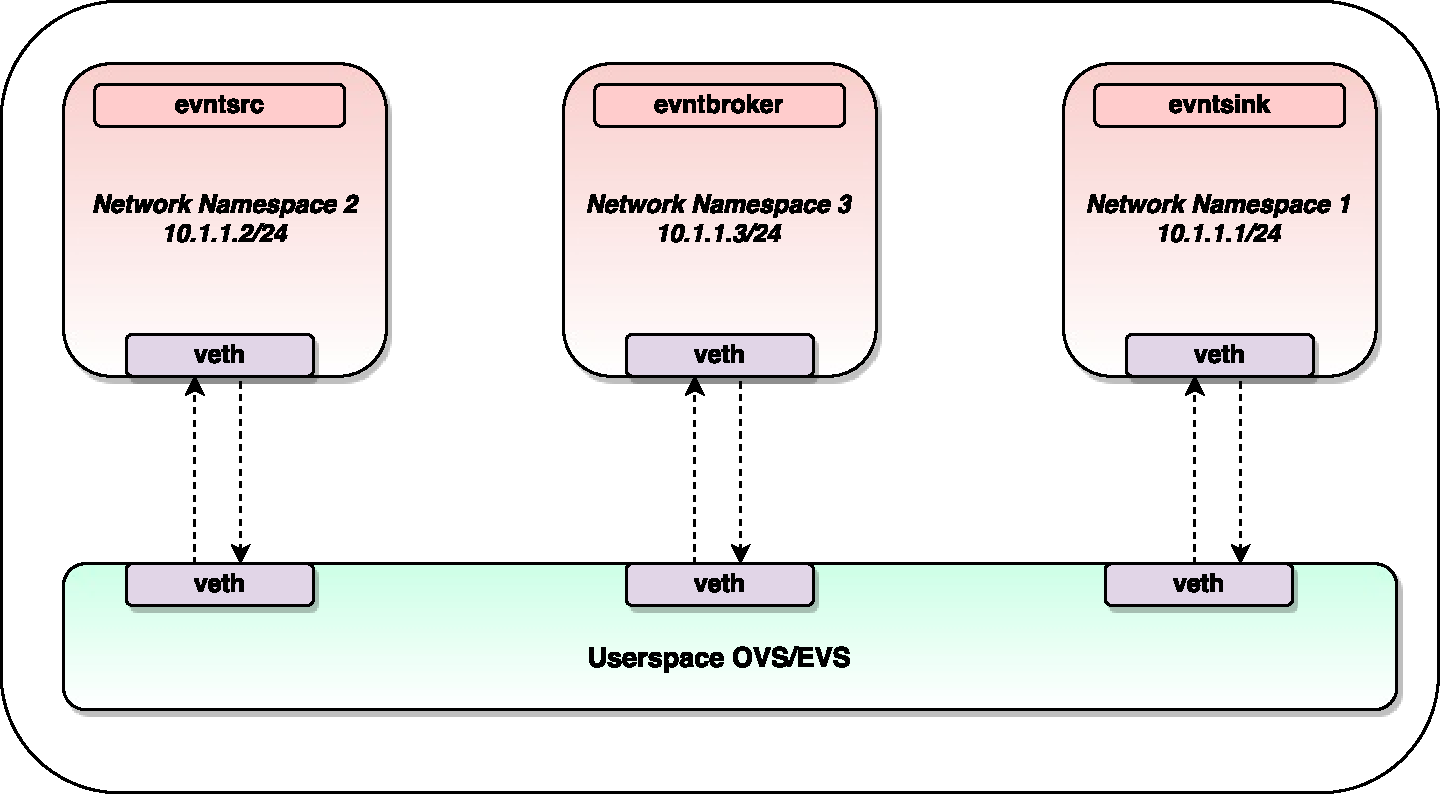
\includegraphics[height=8cm]{nsovs01.pdf}
\end{figure}


\subsection{Set-up Methodology}
In this subsection the steps taken to set up the Network Namespaces bridged on the two userspace bridges is detailed. To begin the set up, it is assumed that the EVS code base is compiled and the ovs-vswitchd daemon and the ovsdb-server are up and running. In addition the modified RYU controler is also running with OpenFlow v1.0.  With this in place, the following steps are taken to set-up the system.
\begin{itemize}
\item To begin the set up, the userspace EVS bridge has to be initialized. \noindent See the following command:
 \begin{lstlisting}[language=bash]
	$ ovs-vsctl add-br br0 -- set bridge br0 datapath_type=netdev \end{lstlisting}
\end{itemize}
\begin{itemize}
	\item The namespaces are set up. In this document, the set up for one namespace is shown.
	\begin{lstlisting}[language=bash]
	$ ip netns add ns1 \end{lstlisting}
\end{itemize}
\begin{itemize}
	\item Two veth pairs of ports are created.
	\begin{lstlisting}[language=bash]
	$ ip link add tap1 type veth peer name ovs-tap1 \end{lstlisting}
\end{itemize}
\begin{itemize}
	\item One end of the created pair is attached to the EVS bridge.
	\begin{lstlisting}[language=bash]
	$ ovs-vsctl add-port br0 ovs-tap1 \end{lstlisting}
\end{itemize}
\begin{itemize}
	\item The other end of the pair is attached to the network namespace.
	\begin{lstlisting}[language=bash]
	$ ip link set tap1 netns ns1 \end{lstlisting}
\end{itemize}
\begin{itemize}
	\item The interface in the network namespace is statically assigned with an ip and both the ends of the pairs are brought up.
	\begin{lstlisting}[language=bash]
	$ ip netns exec ns1 ip link set dev tap1 up
	$ ip netns exec ns1 ip addr add 10.1.1.1/24 dev tap1
	$ ip netns exec ns1 ip link set lo up
	$ ip link set dev ovs-tap1 up \end{lstlisting}
\end{itemize}
\begin{itemize}
	\item The evntsink, evntsrc and evntbroker applications are run on the three namespaces.
	\begin{lstlisting}[language=bash]
	$ ip netns exec ns1 java evntsink
	$ ip netns exec ns2 java evntsrc
	$ ip netns exec ns2 java evntbroker \end{lstlisting}
\end{itemize}

\begin{itemize}
	\item Install the rules onto the EVS bridge to handle the event operations. The API signature for detecting and event of type 'TEST' and redirecting it the evntsink at 10.1.1.1 is shown below:
\begin{lstlisting}[language=json,firstnumber=1]
 {
"dpid": 178974088016461,
"table_id": 0,
"priority": 11112,
"flags": 1,
"match":{
"dl_type":0x0800,
"nw_proto":17,
"nw_dst":"10.1.1.1",
"tp_dst":9877,
"e_type":"TEST"
},
"actions":[{
"type":"set_nw_dst",
"nw_dst": 10.1.1.1
},
{
"type":"NORMAL"
}
]
}
http://localhost:8080/stats/flowentry/add \end{lstlisting}
\end{itemize}

The latency measurements are produced at the evntsink application. It is important to understand the methodology for measurement. Network namespaces are purely separate logical networks. They run on the same CPU and use the Hardware. Technologies such as dockers, linux containers combine facilities provided by network namespaces, process namespaces, file system namespace, IPC namespaces among others with linux control groups to provide virtualization containers. But network namespaces simply provide a logical network stack. To measure the latency, the evntsrc application sends the system timestamp in the payload. The payload follows format specified in figure 4.5. On receiving the packet, the eventsink extracts the timestamp from the payload, computes the difference with current system time. The delta value is aggregated for 1000 UDP packets in each run to give one trial reading of the point-to-point latency. The same methodology is used across all experiments.

\subsection{Performance measurement without event operations}
In this subsection, the evaluation of latency between the evntsrc and evntsink connected without performing any event detection and redirection operation is detailed. Here the EVS bridge performs the role of a standard OVS bridge because no rules specific to events are installed. The packets are sent directly from evntsrc to evntsink without the need for evntbroker. The same exercise is repeated for the standard OVS bridge in order to contrast the performance of the two bridges. The observed results of this analysis are summarized in Figure 5.4. As we can see, the point-to-point latency between evntsrc and evntsink on the EVS bridge is only slightly greater than that of the point-to-point latency of the same on the standard OVS bridge. The slight increase in latency can be attributed to the fact that the EVS bridge performs deep packet inspection per packet to parse and de-serialize the payload data. 
\newline
In addition to point-to-point latency, the bandwidth of the link, and average round trip time (RTT) is measured for both EVS and OVS bridge. To measure the bandwidth of the link, \textit{hperf3} is used and to measure RTT \textit{hping3} is used. As we see in Figure 5.1, EVS bridge is similar to the standard OVS bridge when compared on the parameters of link bandwith and RTT. The bandwidth of the link is  low in both  cases because namespaces are bridged using virtual interfaces and expectedly have low throughput.
\begin{figure}[H]
\centering
\caption{Performance of bridged namespaces}
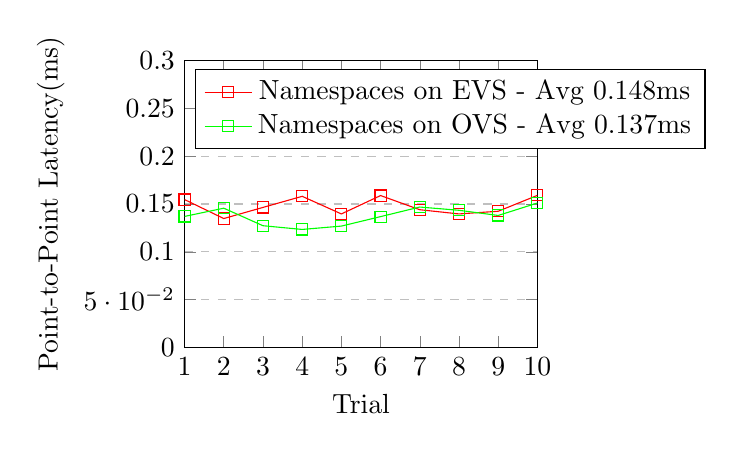
\begin{tikzpicture} [baseline=(current axis.outer east)]
\begin{axis}[
width=0.5\textwidth,
xlabel={Trial},
ylabel={Point-to-Point Latency(ms)},
xmin=1, xmax=10,
ymin=0.00, ymax=0.30,
xtick={1,2,3,4,5,6,7,8,9,10},
ytick={0.00,0.05,0.10,0.15,0.20,0.25,0.30},
legend pos=north west,
ymajorgrids=true,
grid style=dashed,
]
\addplot[
color=red,
mark=square,
]
coordinates {
	(1,0.1546)(2,0.1348)(3,0.1464)(4,0.158)(5,0.1396)(6,0.1588)(7,0.144)(8,0.1396)(9,0.1424)(10,0.159)
};
\addlegendentry{Namespaces on EVS - Avg 0.148ms}
\addplot[
color=green,
mark=square,
]
coordinates {
	(1,0.137)(2,0.1456)(3,0.1273)(4,0.1234)(5,0.1269)(6,0.1368)(7,0.1468)(8,0.1434)(9,0.1380)(10,0.1510)
};
\addlegendentry{Namespaces on OVS - Avg 0.137ms}



\end{axis}
\end{tikzpicture}\hfill
	\begin{tabular} {lrr}
	\toprule
	\hline
	&  OVS Bridge & EVS Bridge  \\ \midrule
	\hline 
	Bandwidth &  154 Mbits/s & 149 Mbits/s  \\ 
	\hline
	Avg RTT & 0.183 ms & 0.180 ms  \\ \bottomrule
	\hline	
\end{tabular}
\end{figure}


\subsection{Performance measurement with event detection and redirection}
In this subsection the performance evaluation of the bridge whilst performing an event detection and redirection operation on a single event type is presented.  For example, Let us say an event with type 'TEST' is sent from evntsrc to the evntbroker. 
This operation is notated as: \begin{equation} D(e.t) \quad | \quad stream,  \end{equation}
where \textit{D} is the detect operation; \newline
\textit{|} denotes the redirect operation; \newline
and \textit{stream} is the logical stream to which the detected event is redirected to. \newline \newline

Whereas other streaming applications may have named stream support, EVS stream redirection is done based on network addresses of the application consuming the event stream. The controller rule installed in EVS corresponding to this operation is:

\begin{lstlisting}[language=json,firstnumber=1]
{
"dpid": 178974088016461,
"table_id": 0,
"priority": 11112,
"flags": 1,
"match":{
"dl_type":0x0800,
"nw_proto":17,
"nw_dst":"10.1.1.1",
"tp_dst":9877,
"e_type":"TEST",
},
"actions":[{
"type":"set_nw_dst",
"nw_dst": 10.1.1.1
},
{
"type":"NORMAL"
}
]
}
http://localhost:8080/stats/flowentry/add \end{lstlisting}

Consider a stream of TEST events where each event has readings from multiple sensors which has to be redirected to another processing engine specifically built for handling these events using an Event Processing language. Such a query is in essence similar to the operation defined in (5.1) and would normally look like:

\begin{verbatim}
INSERT INTO NEWTESTPSTREAM
SELECT * FROM TESTSTREAM
\end{verbatim}

In the EVS bridge, this event of type 'TEST' is detected and redirected to the evntsink using \textit{mod_nw_dst} action rules. Hence the event doesn't go to the evntbroker when EVS bridge is used. As discussed before streams in EVS are identified using network addresses. Named stream support isn't provided. Although it is possible to create custom actions with custom names and make them perform the \textit{mod_nw_dst} actions, in a way mimicking the idea of 'named' streams, this would make a) add more lines of code in the already strong 0.5 million lines of code in OVS, and b) would mean custom action for every stream and thus wouldn't scale.

\begin{figure}[H]
\centering
\caption{Performance of Event Redirection}
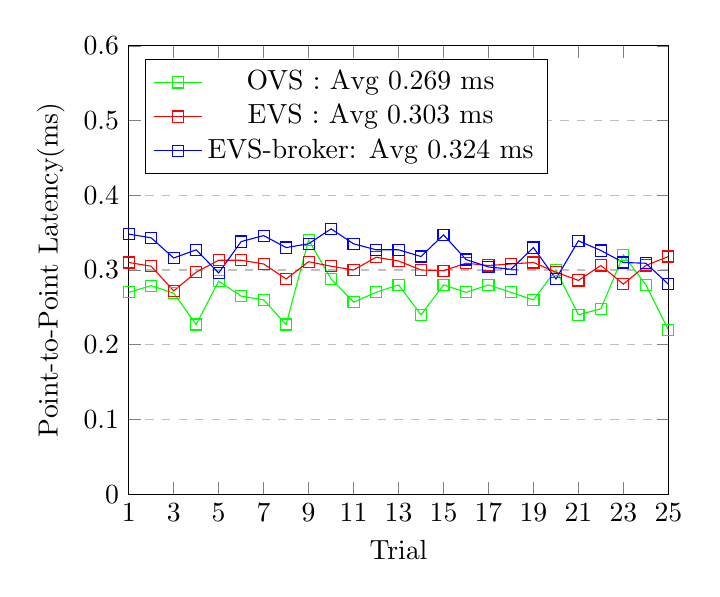
\begin{tikzpicture}
\begin{axis}[
xlabel={Trial},
ylabel={Point-to-Point Latency(ms)},
xmin=1, xmax=25,
ymin=0.00, ymax=0.60,
xtick={1,3,5,7,9,11,13,15,17,19,21,23,25},
ytick={0.00,0.10,0.20,0.30,0.40,0.50,0.60},
legend pos=north west,
ymajorgrids=true,
grid style=dashed,
]

\addplot[
color=green,
mark=square,
]
coordinates {
(1,0.27)
(2,0.279)
(3,0.269)
(4,0.227)
(5,0.285)
(6,0.265)
(7,0.26)
(8,0.227)
(9,0.34)
(10,0.288)
(11,0.257)
(12,0.27)
(13,0.28)
(14,0.24)
(15,0.28)
(16,0.27)
(17,0.28)
(18,0.27)
(19,0.26)
(20,0.3)
(21,0.24)
(22,0.248)
(23,0.32)
(24,0.28)
(25,0.22)
	
};
\addlegendentry{OVS : Avg 0.269 ms}

\addplot[
color=red,
mark=square,
]
coordinates {
	(1,0.31)
	(2,0.305)
	(3,0.272)
	(4,0.297)
	(5,0.313)
	(6,0.313)
	(7,0.308)
	(8,0.288)
	(9,0.311)
	(10,0.305)
	(11,0.3)
	(12,0.317)
	(13,0.312)
	(14,0.3)
	(15,0.299)
	(16,0.309)
	(17,0.306)
	(18,0.308)
	(19,0.31)
	(20,0.297)
	(21,0.286)
	(22,0.306)
	(23,0.281)
	(24,0.306)
	(25,0.318)
	
};
\addlegendentry{EVS : Avg 0.303 ms}

\addplot[
color=blue,
mark=square,
]
coordinates {
	(1,0.348)
	(2,0.343)
	(3,0.316)
	(4,0.327)
	(5,0.296)
	(6,0.338)
	(7,0.346)
	(8,0.33)
	(9,0.335)
	(10,0.355)
	(11,0.335)
	(12,0.327)
	(13,0.327)
	(14,0.318)
	(15,0.347)
	(16,0.314)
	(17,0.304)
	(18,0.301)
	(19,0.33)
	(20,0.288)
	(21,0.339)
	(22,0.326)
	(23,0.31)
	(24,0.309)
	(25,0.281)
	
};
\addlegendentry{EVS-broker: Avg 0.324 ms}

\end{axis}
\end{tikzpicture}
\end{figure}

The same experiment is repeated on the OVS bridge. But in this case, the event with type 'TEST' is simply forwarded to the evntbroker, which proceeds to detect the event and sends it to the relevant evntsink. As we can see in the graph in figure 5.5, the performance of event redirection at the EVS bridge is lower than the performance of event redirection done on an evntbroker, albeit marginally. Even though the EVS bridge prevents the packet from going into the evntbroker and reduces the number of hops for the event packet, the expected improvement in performance is not seen. This can be explained by two factors. One, the redirection in EVS bridge is performed by \textit{mod_tp_dst} or \textit{mod_nw_dst} or \textit{mod_dl_dst} depending on the layer. These Openflow actions modify the event packet and also redirect the individual event packet into the datapath interface, which in case of userspace EVS is dpif-netdev. This additional parsing and lookup balances out the benefits of removing the evntbroker. Two, the EVS bridge employs per packet event de serialization and parsing, which adds some overhead. 

In addition to the above described experiments, the EVS bridge was set up with an evntbroker and evaluated to get a better sense of the performance. In this set up although the EVS bridge is used, the event detection rules are not installed. Instead the events are forwarded to the broker as if operating in the standard OVS mode. This results show far higher latency than the standard OVS bridge and slightly higher latency compared to the EVS bridge running in event processing mode. In the latter case, EVS in event processing mode has two fewer packet hops resulting in lower latency. In the former case, we clearly see that although the OVS bridge and EVS in evntbroker have equal number of packet hops, the per-packet parsing and de-serialization of events, as described before, adds an overhead. By comparing the three results, we get an idea of how much overhead is added by the per-packet event parsing and de-serialization and how much overhead is added by the context switch and the extra packet hops. 

These results provides an interesting insight to the evaluation process in a virtualized environment. In a virtualized environment the costs added by the per-packet processing are going to be similar to the per-packet processing overhead in namespaces, but the costs added by context switch from host to VM , back to host are going to be a lot more expensive. There is more discussion on this topic in section 5.5.

\subsection{Performance measurement with increasing size of event types}
In this subsection an evaluation of the bridge is presented with an increasing size of event types. To do the same, the evntsrc generates events with types ranging from 1 to 9 characters. The analysis was done on the EVS bridge and on the OVS bridge. As seen in the left graph plotted in Figure 5.6, the increasing size of an event type string doesn't result in a linear increase in latency in both the cases. For EVS bridge, this is explained by the fact that Tuple search space classifier of Open vSwitch creates a hash table for every unique combination of inserted flow rule. In the case of this evaluation, one flow rule is added for each run, while increasing the size of event type field in consecutive runs. Additionally, although the event type field matches against a string in the event payload, the match field during flow rule insertion for event type is Hexadecimal value of the string. The rationale behind this approach is that strings within an event payload are serialized into Hexadecimal values on the wire, and since event parsing is part of the packet processing pipeline, keeping the fields as-is avoids the expensive conversion, thus reducing the overhead on the processing pipeline. 

In case of the OVS bridge, the broker does a simple string match, and increasing the size of the string makes little to no difference. It would therefore be interesting to see how adding additional event types would impact the performance of the two bridges. 

\begin{figure}[H]
	
    \noindent\hrulefill

\noindent
\caption{Changing Size and Number of Event Types}
	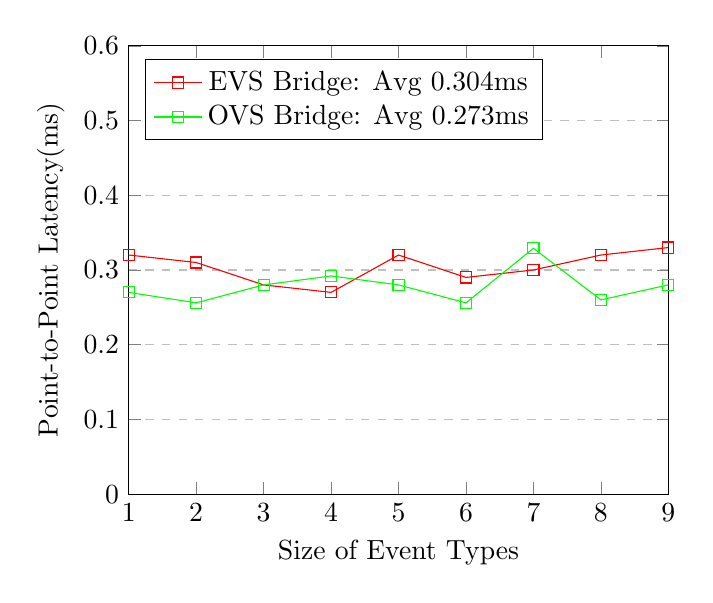
\begin{tikzpicture} 
	\begin{axis}[
	xlabel={Size of Event Types},
	ylabel={Point-to-Point Latency(ms)},
	xmin=1, xmax=9,
	ymin=0.00, ymax=0.60,
	xtick={1,2,3,4,5,6,7,8,9},
	ytick={0.00,0.10,0.20,0.30,0.40,0.50,0.60},
	legend pos=north west,
	ymajorgrids=true,
	grid style=dashed,
	]
	\addplot[
	color=red,
	mark=square,
	]
	coordinates {
		(1,0.32)(2,0.31)(3,0.28)(4,0.27)(5,0.32)(6,0.29)(7,0.30)(8,0.32)(9,0.33)
	};
	\addlegendentry{EVS Bridge: Avg 0.304ms}
	
		\addplot[
	color=green,
	mark=square,
	]
	coordinates {
		(1,0.27)(2,0.256)(3,0.28)(4,0.292)(5,0.28)(6,0.256)(7,0.329)(8,0.26)(9,0.28)
	};
	\addlegendentry{OVS Bridge: Avg 0.273ms}
	
	\end{axis}
	\end{tikzpicture} 
       \hfil
	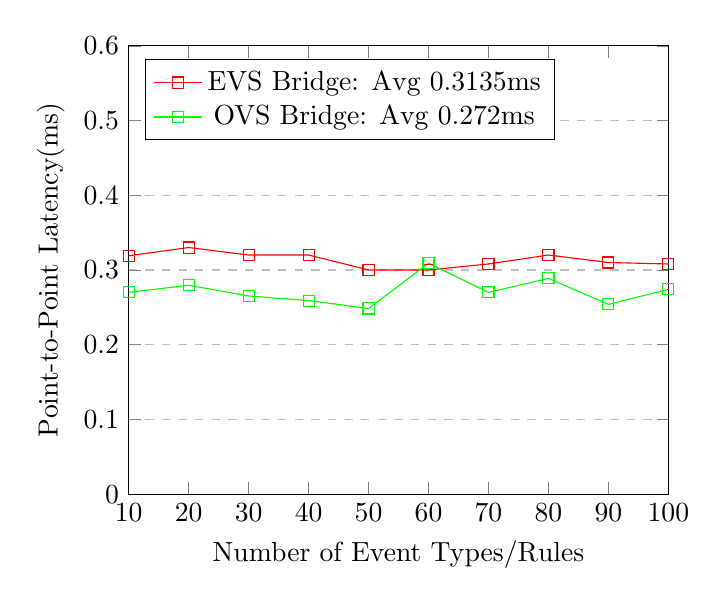
\begin{tikzpicture} 
\begin{axis}[
xlabel={Number of Event Types/Rules},
ylabel={Point-to-Point Latency(ms)},
xmin=10, xmax=100,
ymin=0.00, ymax=0.60,
xtick={10,20,30,40,50,60,70,80,90,100},
ytick={0.00,0.10,0.20,0.30,0.40,0.50,0.60},
legend pos=north west,
ymajorgrids=true,
grid style=dashed,
]
\addplot[
color=red,
mark=square,
]
coordinates {
	(10,0.319)(20,0.33)(30,0.32)(40,0.32)(50,0.30)(60,0.30)(70,0.308)(80,0.32)(90,0.31)(100,0.308)
};
\addlegendentry{EVS Bridge: Avg 0.3135ms}

\addplot[
color=green,
mark=square,
]
coordinates {
	(10,0.27)(20,0.2795)(30,0.265167)(40,0.259)(50,0.2485)(60,0.309)(70,0.270)(80,0.2887)(90,0.254)(100,0.274)
};
\addlegendentry{OVS Bridge: Avg 0.272ms}

\end{axis}
\end{tikzpicture}
\end{figure}	

\subsection{Performance measurement with increasing number of event types }	
In addition to size of event types, the number of event types sent to the EVS bridge were also increased to measure the impact on latency. Each event type is handled by one rule in EVS bridge, so to handle 100 event types and redirect them to evntsink the EVS bridge was set up with 100 rules. As see in the right graph in Figure 5.6, an increase in the number of event types/rules does not affect the performance of the EVS bridge. This is because the number of flow rules remain constant, only the actions on each flow rule is modified to increase filtered events. And since the Tuple Space Search Classifier only adds an additional Hashtable when there is an new combination of fields entered as a flow rule, even increasing the number flow rules, as long as they have the same match fields would not result in additional lookups.
The same two experiment set ups were repeated for the standard OVS bridge, with an evntbroker responsible for handling and forwarding the event types to the evntsrc. EVS bridge and OVS bridge performed similarly in this regard showcasing the potential of the EVS bridge in real-world scenarios.



\begin{figure}[H]
	\centering
	\caption{Performance of Event Filtering}
	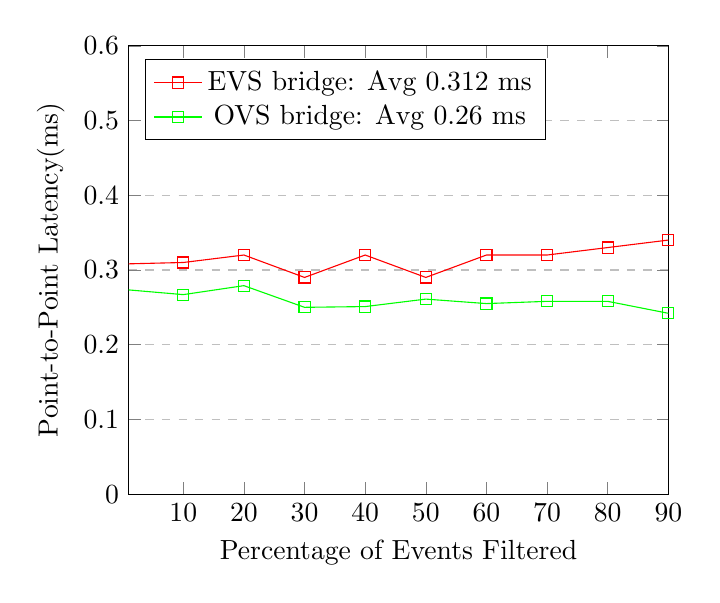
\begin{tikzpicture}
	\begin{axis}[
	xlabel={Percentage of Events Filtered},
	ylabel={Point-to-Point Latency(ms)},
	xmin=1, xmax=90,
	ymin=0.00, ymax=0.60,
	xtick={10,20,30,40,50,60,70,80,90},
	ytick={0.00,0.10,0.20,0.30,0.40,0.50,0.60},
	legend pos=north west,
	ymajorgrids=true,
	grid style=dashed,
	]
	\addplot[
	color=red,
	mark=square,
	]
	coordinates {
		(0,0.308)
		(10,0.31)
		(20,0.32)
		(30,0.29)
		(40,0.32)
		(50,0.29)
		(60,0.32)
		(70,0.32)
		(80,0.33)
		(90,0.34)
	};
	\addlegendentry{EVS bridge: Avg 0.312 ms}
	
	\addplot[
	color=green,
	mark=square,
	]
	coordinates {
		(0,0.274)
		(10,0.267)
		(20,0.279)
		(30,0.25)
		(40,0.251)
		(50,0.261)
		(60,0.255)
		(70,0.258)
		(80,0.258)
		(90,0.242)
	};
	\addlegendentry{OVS bridge: Avg 0.26 ms}
	
	\end{axis}
	\end{tikzpicture}
\end{figure}	

\subsection{Performance measurement with increasing percentage of filtered event types}
In this subsection the performance evaluation of the EVS bridge with an increasing percentage of filtered event types is presented. The evntsrc is configured to generate 100 random event types, addressed to the evntbroker. The EVS bridge initially is configured with flow rules to send through all the events. At this stage the setup is similar to the sub-section 5.4.3 with 100 event types and flow rules. In the next stage 10\% of the event types are filtered with an additional 10\% added subsequently until all the events are filtered. The same experiment is repeated for the standard OVS bridge. In the case of OVS bridge, the filtering is done in the evntbroker. 
\newline
As seen in the graph plotted in Figure 5.7, both EVS and OVS perform very similarly when the percentage of event filters is increased. This  experiment however does not showcase the benefits of event filtering in EVS. Because the measurements are taken only when the event is delivered to the evntsink. And for the event to be delivered to the evntsink, it must first be redirected by the EVS bridge using the expensive \textit{mod} actions. 





\subsection{Performance measurement of event attributes detection and redirection}
In this subsection the performance evaluation of the EVS bridge is presented when event attributes are detected and redirected. The results are contrasted to the measurements produced when similar attributes are detected and redirected using the evntbroker on the OVS bridge. To do the set up for the experiment, rules are installed into the EVS bridge to detect event attributes. When the events with the given attribute or pattern of attributes are detected, the events are redirected to the evntsink. All the other events are filtered out. 

\subsubsection{Detect operation on one attribute}

First, the rule for detecting event type and  a single event attribute is considered. This operation is notated by: \begin{equation} D(e.t  \wedge e.a_1) \quad | \quad stream,  \end{equation}
where \textit{D} is the detect operation; \newline
\textit{e.t} is the event type; \newline
\textit{e.a1} is the first event attribute; \newline
\textit{|} denotes the redirect operation; \newline
and \textit{stream} is the logical stream to which the detected event is redirected to. \newline \newline

Whereas other streaming applications may have named stream support, EVS stream redirection is done based on network addresses of the application consuming the event stream. The controller rule installed in EVS corresponding to this operation is:

\begin{lstlisting}[language=json,firstnumber=1]
{
"dpid": 178974088016461,
"table_id": 0,
"priority": 11112,
"flags": 1,
"match":{
"dl_type":0x0800,
"nw_proto":17,
"nw_src":"10.1.1.2"
"nw_dst":"10.1.1.3",
"tp_dst":9877,
"e_type":"TEMP",
"e_attr1":80,
},
"actions":[{
"type":"set_nw_dst",
"nw_dst": 10.1.1.1
},
{
"type":"NORMAL"
}
]
}
http://localhost:8080/stats/flowentry/add \end{lstlisting}

This is similar to the INSERT INTO clause provided by many Event Processing Languages, where the events from an event stream are filtered based on a value and forwarded into another event stream. In this case, the new event stream is the the stream of events handed over to the application listening on port 9877. Consider a stream of temperature events where each event has readings from multiple sensors. The operation at (5.2) is semantically similar to the below Event-Processing  query:

\begin{verbatim}
INSERT INTO NEWTEMPSTREAM
SELECT * FROM TEMPSTREAM
WHERE DEVICE_1.VALUE = 80
\end{verbatim}

As seen in Figure 5.8, the latency caused by performance of the operation notated in (5.2) in the EVS bridge is marginal higher than the latency observed on the standard OVS bridge by the order of 0.02 ms. When the same operation was evaluated on the EVS bridge operating in standard mode, the latency observed was marginally higher than the OVS bridge by a order 0.03 ms. This is effectively the latency added by per-packet event processing. 

\pgfplotstableread[row sep=\\,col sep=&]{
	Operations & OVS & EVS & EVS-broker \\
	5.1     & 0.27  & 0.30  & 0.32  \\
	5.2     & 0.27 & 0.29  & 0.313  \\
	5.3    & 0.28 & 0.29 & 0.318 \\
	5.4    & 0.29 & 0.3 & 0.308 \\
}\mydata



\begin{figure}[H]
	\centering
	\caption{Performance of Event attribute match operations}
	\begin{tikzpicture}
	\begin{axis}[
	ybar,
	xlabel={Operations},
	ylabel={Point-to-Point Latency(ms)},
	symbolic x coords={5.1,5.2,5.3,5.4},
    xtick=data,
	nodes near coords,
	    legend style={at={(0.5,1)},
		anchor=north,legend columns=-1},
	]
	\addplot[fill=green] table[x=Operations,y=OVS]{\mydata};
	\addplot[fill=red ] table[x=Operations,y=EVS]{\mydata};
	\addplot[fill=blue] table[x=Operations,y=EVS-broker]{\mydata};
    \legend{OVS, EVS, EVS-broker}
	\end{axis}
	\end{tikzpicture}
\end{figure}

\subsubsection{Detect operation on two disjunct attributes}

The next operation considered for evaluation is notated by:

\begin{equation}D(e.t  \wedge (e.a_1 \vee e.a_2)) \quad | \quad stream, \end{equation}
where \textit{D} is the detect operation; \newline
\textit{e.t} is the event type; \newline
\textit{e.a1} is the first event attribute; \newline
\textit{e.a2} is the second event attribute;
\textit{|} denotes the redirect operation; \newline
and \textit{stream} is the logical stream to which the detected event is redirected to. \newline \newline

The controller installs an additional rule - seen below - in addition to the one above, to perform this operation:
\begin{lstlisting}[language=json,firstnumber=1]
{
"dpid": 178974088016461,
"table_id": 0,
"priority": 11112,
"flags": 1,
"match":{
"dl_type":0x0800,
"nw_proto":17,
"nw_src":"10.1.1.2"
"nw_dst":"10.1.1.3",
"tp_dst":9877,
"e_type":"TEMP",
"e_attr2":80,
},
"actions":[{
"type":"set_nw_dst",
"nw_dst": 10.1.1.1
},
{
"type":"NORMAL"
}
]
}
http://localhost:8080/stats/flowentry/add \end{lstlisting}

Drawing parallel to an Event Processing Language, the operation at (5.2) is similar to:

\begin{verbatim}
INSERT INTO NEWTEMPSTREAM
SELECT * FROM TEMPSTREAM
WHERE DEVICE_1.VALUE = 80 OR DEVICE_2.VALUE=80
\end{verbatim}

As we seen in Figure 5.8, the execution of this operation follows the trends observed for operations 5.1 ad 5.2. No remarkable overhead was added on the EVS bridge, despite the addition of the rule. The reason for this is clearly explained in section 5.4.6.


\subsubsection{Detect operation on two conjunct attributes}
The next operation considered for evaluation is notated by:

\begin{equation}D(e.t  \wedge (e.a_1 \wedge e.a_2)) \quad | \quad stream, \end{equation}
where \textit{D} is the detect operation; \newline
\textit{e.t} is the event type; \newline
\textit{e.a1} is the first event attribute; \newline
\textit{e.a2} is the second event attribute;
\textit{|} denotes the redirect operation; \newline
and \textit{stream} is the logical stream to which the detected event is redirected to. \newline \newline

The controller installs one rule - seen below - to perform this operation:
\begin{lstlisting}[language=json,firstnumber=1]
{
"dpid": 178974088016461,
"table_id": 0,
"priority": 11112,
"flags": 1,
"match":{
"dl_type":0x0800,
"nw_proto":17,
"nw_src":"10.1.1.2"
"nw_dst":"10.1.1.3",,
"tp_dst":9877,
"e_type":"TEMP",
"e_attr1":80,
"e_attr2":80,
},
"actions":[{
"type":"set_nw_dst",
"nw_dst": 10.1.1.1
},
{
"type":"NORMAL"
}
]
}
http://localhost:8080/stats/flowentry/add \end{lstlisting}

Drawing parallel to an Event Processing Language, the operation at (5.2) is similar to:

\begin{verbatim}
INSERT INTO NEWTEMPSTREAM
SELECT * FROM TEMPSTREAM
WHERE DEVICE_1.VALUE = 80 AND DEVICE_2.VALUE=80
\end{verbatim}

As seen in Figure 5.8, and similar to the case of disjunction operation (5.3), the execution of the conjunction operation in the EVS bridge does not add any remarkable point-to-point latency. And as expected, the EVS-broker has the worst perfomance, because of the added processing and packet hops.

\subsubsection{Network Traffic Monitoring for the event detection and redirection operations}
For all the operations defined through 5.1 to 5.4, the traffic in the network was monitored both in the case of OVS and EVS bridge. The system was set up to send a flow of 100000 UDP packets from the eventsrc to the evntsink. The traffic characteristics observed on the six interfaces are shown in Table 5.2. It can be observed that the EVS bridge avoids using the interfaces related to namespace 3 completely for the flow. That is a 33\% reduction in traffic for single staged event processing.

\begin{center}
	\captionof{table}{Network traffic on Namespaces} \label{tab:title} 
	\begin{tabular}{ |c|c|c| }
		\hline
		 \textbf{Interface} &  \textbf{OVS Bridg}e &  \textbf{EVS Bridge} \\\toprule
		\hline
		Hypervisor - tap1 & Tx-100000 & Tx-100000  \\
		\hline 
		Namespace1 - tap1 & Rx-100000 & Rx-100000 \\
		\hline		
		Hypervisor - tap2 &  Rx-100000 & Rx-100000  \\ 
		\hline
		Namespace2 - tap2 & Tx-100000 & Tx-100000 \\
		\hline		
		Hypervisor - tap3 & Rx-100000, Tx-100000 & 0  \\ 
		\hline
		Namespace3 - tap3 & Rx-100000, Tx-100000 & 0 \\
		\hline
	\end{tabular}
\end{center}


\subsection{Performance measurement of compare operations on event attributes}
In this subsection, the performance of the comparison operations on the event attributes is presented. This class of operations perform a binary operation on the event attribute value. The evaluation of two compare operators which have been implemented- \textit{Greater than or equal to (>=)}, \textit{Less than or equal to (<=)} - is detailed. 

\subsubsection{Greater than or equal to operator}
The operation supported by Greater than or equal to operator is notated by:
\begin{equation}D(e.t  \wedge (e.a_1 >= value) \quad | \quad filter, \end{equation}
where \textit{D} is the detect operation; \newline
\textit{e.t} is the event type; \newline
\textit{e.a1} is the first event attribute; \newline
\textit{value} is the integer value to be compared with; \newline
\textit{|} denotes the redirect operation; \newline
and \textit{fliter} is the denotation for filtering of the event. \newline \newline
\begin{lstlisting}[language=json,firstnumber=1]
{
	"dpid": 178974088016461,
	"table_id": 0,
	"priority": 11112,
	"flags": 1,
	"match":{
		"dl_type":0x0800,
		"nw_proto":17,
		"nw_dst":"10.1.1.2",
		"nw_dst":"10.1.1.1",
		"tp_dst":9877,
		"e_type":"TEMP",
	},
	"actions":[{
		"type":"set_max",
		"value": 100
	},
	{
		"type":"NORMAL"
	}
	]
}
http://localhost:8080/stats/flowentry/add \end{lstlisting}

Which in the perspective of event query languages can be represented as:

\begin{verbatim}
DROP FROM TEMPSTREAM
WHERE DEVICE_1.VALUE >= 100
\end{verbatim}

The operation at (5.5) can be used with conjunction operation on event attribute2.
\begin{equation}D(e.t  \wedge ((e.a_1 >= value) \wedge e_2 )\quad | \quad filter, \end{equation}

or with the disjunction operation on attribute2.

\begin{equation}D(e.t  \wedge ((e.a_1 >= value) \vee e_2 )\quad | \quad filter, \end{equation}

 The Less than or equal to operator is introduced next and the evaluation discussion of the two operators is presented together at the end of the subsection.

\subsubsection{Less than or equal to operator}
The operation supported by Greater than or equal to operator is notated by:
\begin{equation}D(e.t  \wedge (e.a_1 <= value) \quad | \quad filter, \end{equation}
where \textit{D} is the detect operation; \newline
\textit{e.t} is the event type; \newline
\textit{e.a1} is the first event attribute; \newline
\textit{value} is the integer value to be compared with; \newline
\textit{|} denotes the redirect operation; \newline
and \textit{fliter} is the denotation for filtering of the event. \newline \newline
\begin{lstlisting}[language=json,firstnumber=1]
{
"dpid": 178974088016461,
"table_id": 0,
"priority": 11112,
"flags": 1,
"match":{
"dl_type":0x0800,
"nw_proto":17,
"nw_dst":"10.1.1.2",
"nw_dst":"10.1.1.1",
"tp_dst":9877,
"e_type":"TEMP",
},
"actions":[{
"type":"set_min",
"value": 100
},
{
"type":"NORMAL"
}
]
}
http://localhost:8080/stats/flowentry/add \end{lstlisting}

Which in the perspective of event query languages can be represented as:

\begin{verbatim}
DROP FROM TEMPSTREAM
WHERE DEVICE_1.VALUE <= 100
\end{verbatim}

The operation at (5.8) can be used with conjunction operation on event attribute2.
\begin{equation}D(e.t  \wedge ((e.a_1 <= value) \wedge e_2 )\quad | \quad filter, \end{equation}

or with the disjunction operation on attribute2.

\begin{equation}D(e.t  \wedge ((e.a_1 <= value) \vee e_2 )\quad | \quad filter, \end{equation}

The attr_cmp action defined in section 4.6.7 internal implements the {<,>,=} operators, the performance observed for the set_min, set_max operators can be generalized for the class of compare operations defined in section 4.6.7. Hence For evaluation purposes only the set_min and set_max operators defined in (5.5) and (5.8) are considered. 

\subsubsection{Performance of compare Operations}
In this subsection, the performance of the compare operations defined in section 4.6.7 is presented. First, the evaluation  of rules defined in (5.5) and (5.8) is presented when only positive values are sent to the system. This evaluation is done in order to understand the rule performance is general and to see if the rule in itself creates a bottleneck in performance. For example, for a set_min:100 rule, only events of type "TEMP" and with values greater than 100 are sent. In this case, each event is forwarded by the rule and none of the events are dropped. The same test was repeated for the set_max:100 operator but this time by passing values less than 100. This test is not intended to test the accuracy of the rules, but only to check if the rules with additional operations add an overhead. The performance is plotted in Figure 5.9 and is contrasted with the inter-namespace switching results provided in section 5.4.2, figure 5.4. As it can be seen, the rules for the two operations do not add a significant overhead and are comparable to the performance of the EVS bridge with inter-namespace switching based on event type attribute.
\begin{figure}[H]
	\centering
	\caption{Comparator Performance}
	\begin{tikzpicture} [baseline=(current axis.outer east)]
	\begin{axis}[
	width=0.5\textwidth,
	xlabel={Trial},
	ylabel={Point-to-Point Latency(ms)},
	xmin=1, xmax=10,
	ymin=0.00, ymax=0.30,
	xtick={1,2,3,4,5,6,7,8,9,10},
	ytick={0.00,0.05,0.10,0.15,0.20,0.25,0.30},
	legend pos=north west,
	ymajorgrids=true,
	grid style=dashed,
	]
	\addplot[
	color=red,
	mark=square,
	]
	coordinates {
		(1,0.1546)(2,0.1348)(3,0.1464)(4,0.158)(5,0.1396)(6,0.1588)(7,0.144)(8,0.1396)(9,0.1424)(10,0.159)
	};
	\addlegendentry{Namespaces on EVS - Avg 0.148ms}
	\addplot[
	color=green,
	mark=square,
	]
	coordinates {
		(1,0.137)(2,0.1456)(3,0.1273)(4,0.1234)(5,0.1269)(6,0.1368)(7,0.1468)(8,0.1434)(9,0.1380)(10,0.1510)
	};
	\addlegendentry{Namespaces on OVS - Avg 0.137ms}
			\addplot[
	color=blue,
	mark=square,
	]
	coordinates {
		(1,0.1699)(2,0.1453)(3,0.1456)(4,0.1456)(5,0.158)(6,0.147)(7,0.163)(8,0.154)(9,0.142)(10,0.143)
		
	};
	\addlegendentry{EVS - set_max - Avg 0.151ms}
	
	\addplot[
	color=yellow,
	mark=square,
	]
	coordinates {
		(1,0.153)(2,0.158)(3,0.147)(4,0.16)(5,0.149)(6,0.149)(7,0.143)(8,0.154)(9,0.152)(10,0.16)
	};
	\addlegendentry{EVS - set_min - Avg 0.152ms}	
	
	
	\end{axis}
	\end{tikzpicture}\hfill

\end{figure}


\subsection{Evaluating for accuracy - compare operations}
In the previous subsection, the performance of the comparision operations were measured only with positive test inputs where none of the events are dropped. But when random values are sent as attributes, the compare operations fail to perform the role they are designed for accurately. This is because of the megaflow cache design of the Open vSwitch. The cross product of all the active flows in the userspace OpenFlow tables are cached in the megaflow table. And as long as the incoming flow matches with an entry in the megaflow table, the learnt action is applied. This makes compare actions tricky to implement. These actions are conditional, i.e if the expression specified by the action evaluates to TRUE, the forwarding action is applied, or else the drop action (or a lack of action) is applied. So when a set_max:100 action is evaluated for the first event, the value for event attribute is extracted; for the ease of discussion let us consider 90 to be this value. Therefore, the set_max action evaluates to TRUE, after which the packet is sent to the learnt port based on the 'nw_dst' address. This flow is now cached in the megaflow table with the learnt output port.
\begin{figure}[H]
	\centering
	\caption{Megaflow cache}
	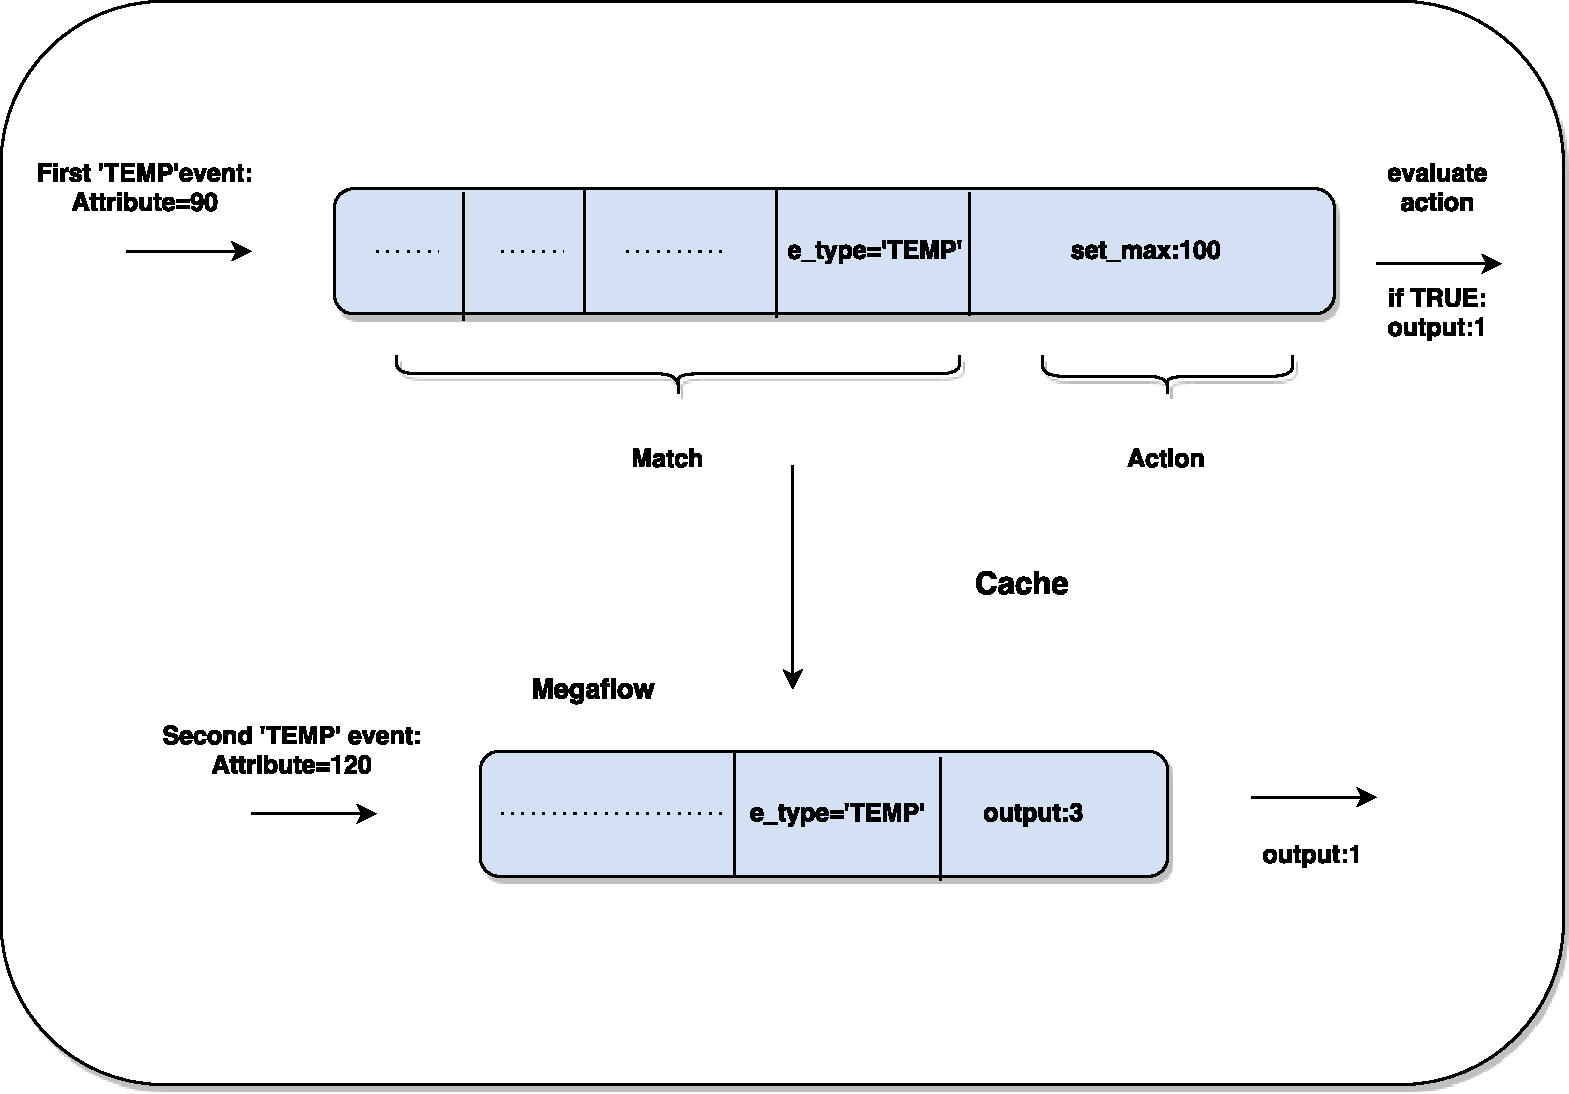
\includegraphics[height=7cm]{learnandcache.pdf}
\end{figure}
The subsequent events are now looked-up in the megaflow cache, and the cached forwarding action is applied. Hence once the events start hitting the megaflow table, there is no opportunity for attribute evaluation. Open vswitch implements a re-validator thread which evicts the inactive flows or to update the recently changed flows. The compare operations from this perspective can be viewed as flows which need to be refreshed after every flow hit. By default the cache revalidation happens every 10 seconds. So if an event of type 'TEMP' hits the compare operator rule once in 10 seconds, the operation is evaluated accurately. However this is not ideal. Hence different ways to reduce this flow hit rate are explored. Open vSwitch provides options to configure the revalidation of the cache.\newline

\subparagraph*{Disabled-Megaflow}
The first approach is to disable-megaflow, using the below command.

	\begin{lstlisting}[language=bash]
$ ovs-appctl upcall/disable-megaflows \end{lstlisting}

After having disabled megaflows, the evaluation to determine the accuracy and performance of the compare operations was performed. The rule installed for this evaluation was:

\begin{lstlisting}[language=json,firstnumber=1]
{
"dpid": 178974088016461,
"table_id": 0,
"priority": 11112,
"flags": 1,
"match":{
"dl_type":0x0800,
"nw_proto":17,
"nw_dst":"10.1.1.2",
"nw_dst":"10.1.1.1",
"tp_dst":9877,
"e_type":"TEMP",
},
"actions":[{
"type":"set_max",
"value": 5
},
{
"type":"NORMAL"
}
]
}
http://localhost:8080/stats/flowentry/add \end{lstlisting}

The results are monitored such that only values greater than 5 are filtered by the EVS bridge, and values less than 5 are allowed through. To test this, the evntsrc is configured to generate events of type 'TEMP', such that every odd iteration generate a value greater than 5 and every even iteration generates a value less than 5. The evntsink counts any unexpected value greater than 5 received as a miss, and reports at the end of the test. 

Another additional parameter that is set up is the frequency of the rule hit. As discussed before, by default Open vSwitch evicts idle megaflow rule every 10 seconds. With the megaflow disabled, this frequency of rule hit was configured by increasing the sleep time of the evntsrc application. This was done in order to measure the accuracy when the frequency is high. This also gives a good indicator of the frequency of rule hit that can be tolerated whilst having the highest accuracy. The results are plotted in Figure 5.11


\begin{figure}[H]		
	
	\caption{Accuracy and latency measure of compare operations with disabled megaflows}
	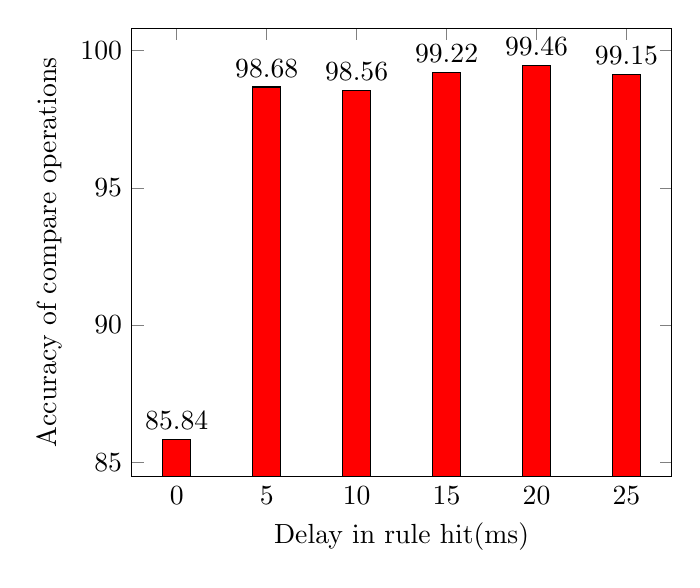
\begin{tikzpicture}
	\begin{axis}[
	xlabel={Delay in rule hit(ms)},
	ylabel={Accuracy of compare operations},
	symbolic x coords={0,5,10,15,20,25},
	xtick=data,
	nodes near coords,
	legend style={at={(0.5,1)},
		anchor=north,legend columns=-1},
	]
	\addplot[ybar,fill=red] coordinates {
		(0,85.84)
		(5,98.68)
		(10,98.56)
		(15,99.22)
		(20,99.46)
		(25,99.15)
	};
	\end{axis}
	\end{tikzpicture}
	\hfil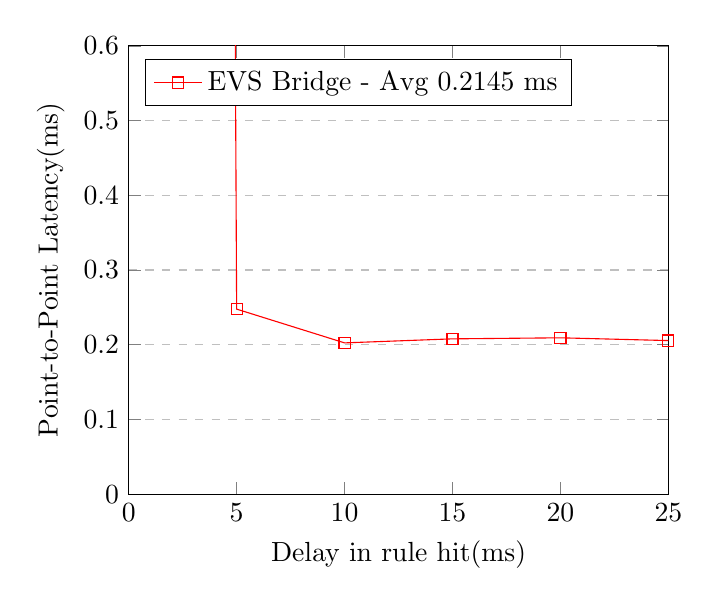
\begin{tikzpicture} 
\begin{axis}[
xlabel={Delay in rule hit(ms)},
ylabel={Point-to-Point Latency(ms)},
xtick=data,
xmin=0, xmax=25,
ymin=0.00, ymax=0.6,
xtick={0,5,10,15,20,25},
ytick={0.00,0.10,0.20,0.30,0.40,0.50,0.60,1,10,20,30},
legend pos=north west,
ymajorgrids=true,
grid style=dashed,
]
\addplot[
color=red,
mark=square,
]
coordinates {
	(0,29.27)(5,0.2476)(10,0.2024)(15,0.2078)(20,0.2092)(25,0.2055)
};
\addlegendentry{EVS Bridge - Avg 0.2145 ms}
\end{axis}
\end{tikzpicture}
\end{figure}


As it can be observed from Figure 5.11, when the compare rule is hit without any delay, the accuracy is at a mere 85.84\% and the latency is measured to be 29.27 ms. But as delay is introduced to the rule hit parameter, the accuracy and latency normalizes to 99\% with 0.21 ms latency. It is to be noted that even the 0.21 ms latency is quite high compared to 0.151 ms and 0.152 ms latency achieved (plotted in Figure 5.9) for set_min and set_max operators with enabled megaflow. This is because in the graph plotted in Figure 5.9, accuracy is not a considered parameter for evaluation and thereby with enabled megaflow caching, the lookup of the rules is much faster and the compare operation is not evaluated for each event. 

\subparagraph*{Configure Max-idle time}
The second approach is to configure the maximum idle time for each flow using:

	\begin{lstlisting}[language=bash]
$ ovs-vsctl --no-wait set Open_vSwitch . other_config:max-idle=1 \end{lstlisting}

Unlike disabling megaflows entirely, this configuration ensures that any flow rule which is idle for more than 1 ms is evicted. The results are plotted in Figure 5.12. As it can be seen, the flow rule accuracy reached 100\% when the delay is 10 ms. This is because the re-validator needs a few milliseconds to evict the idle rules. In this set up the average point-to-point latency hovered around 0.183 ms, which is higher than the 0.151 ms reported in Figure 5.9, but lower than the 0.21 ms observed and plotted in Figure 5.11.


\begin{figure}[H]		
	
	\caption{Accuracy and latency measure of compare operations with flow max idle time=1}
	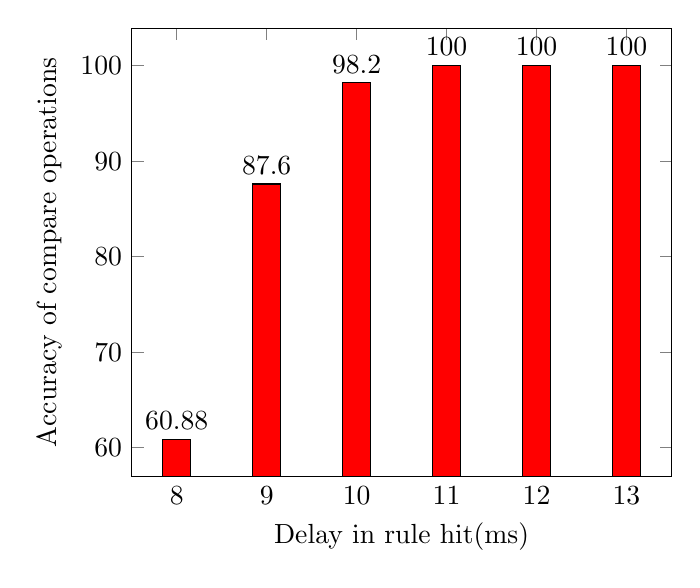
\begin{tikzpicture}
	\begin{axis}[
	xlabel={Delay in rule hit(ms)},
	ylabel={Accuracy of compare operations},
	symbolic x coords={8,9,10,11,12,13},
	xtick=data,
	nodes near coords,
	legend style={at={(0.5,1)},
		anchor=north,legend columns=-1},
	]
	\addplot[ybar,fill=red] coordinates {
		(8,60.88)
		(9,87.6)
		(10,98.2)
		(11,100)
		(12,100)
		(13,100)
	};
	\end{axis}
	\end{tikzpicture}
	\hfil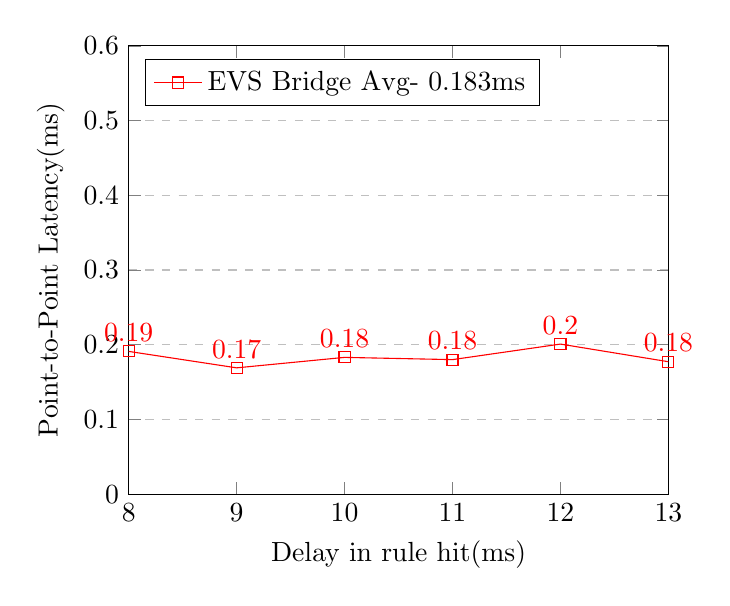
\begin{tikzpicture} 
	\begin{axis}[
	xlabel={Delay in rule hit(ms)},
	ylabel={Point-to-Point Latency(ms)},
	xtick=data,
	xmin=8, xmax=13,
	ymin=0.00, ymax=0.6,
	xtick={8,9,10,11,12,13},
	ytick={0.00,0.10,0.20,0.30,0.40,0.50,0.60},
	legend pos=north west,
	ymajorgrids=true,
	grid style=dashed,
	nodes near coords,
	]
	\addplot[
	color=red,
	mark=square,
	]
	coordinates {
		(8,0.191)(9,0.169)(10,0.183)(11,0.18)(12,0.2008)(13,0.1772)
	};
	\addlegendentry{EVS Bridge Avg- 0.183ms}
	\end{axis}
	\end{tikzpicture}
\end{figure}

 The results from the above experiment show that even though the max-idle time is set at 1 ms, the accuracy is at the peak if the flow hit frequency is around 10 ms. To monitor the change in accuracy and find the best rule hit delay with lowest point-to-point latency, the experiment was repeated with a max-idle time set as 5 ms.

	\begin{lstlisting}[language=bash]
$ ovs-vsctl --no-wait set Open_vSwitch . other_config:max-idle=5 \end{lstlisting}

The results shown in Figure 5.13 shows that when the idle flows are evicted every 5 ms, the ideal rule delay hit is observed at 12 ms where the accuracy is 99.96\% with an average point-to-point latency of 0.2ms.

\begin{figure}[H]		
	
	\caption{Accuracy and latency measure of compare operations with flow max idle time=5}
	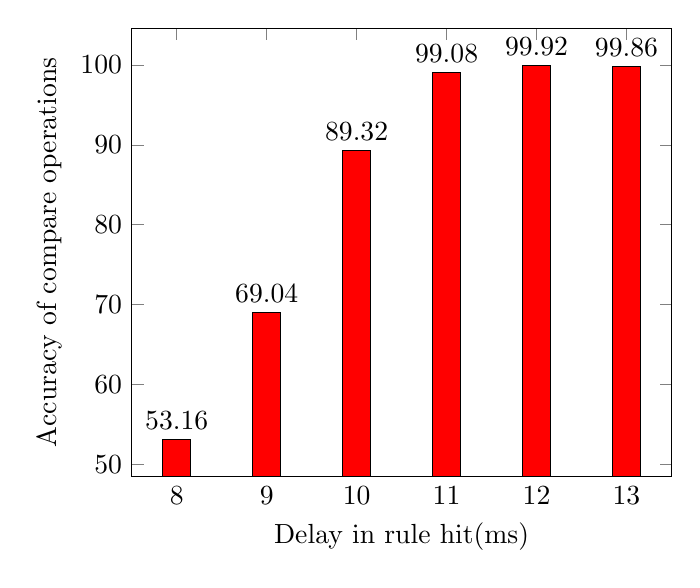
\begin{tikzpicture}
	\begin{axis}[
	xlabel={Delay in rule hit(ms)},
	ylabel={Accuracy of compare operations},
	symbolic x coords={8,9,10,11,12,13,14,15},
	nodes near coords,
	legend style={at={(0.5,1)},
		anchor=north,legend columns=-1},
	]
	\addplot[ybar,fill=red] coordinates {
		
		(8,53.16)
		(9,69.04)
		(10,89.32)
		(11,99.08)
		(12,99.92)
		(13,99.86)
	};
	\end{axis}
	\end{tikzpicture}
	\hfil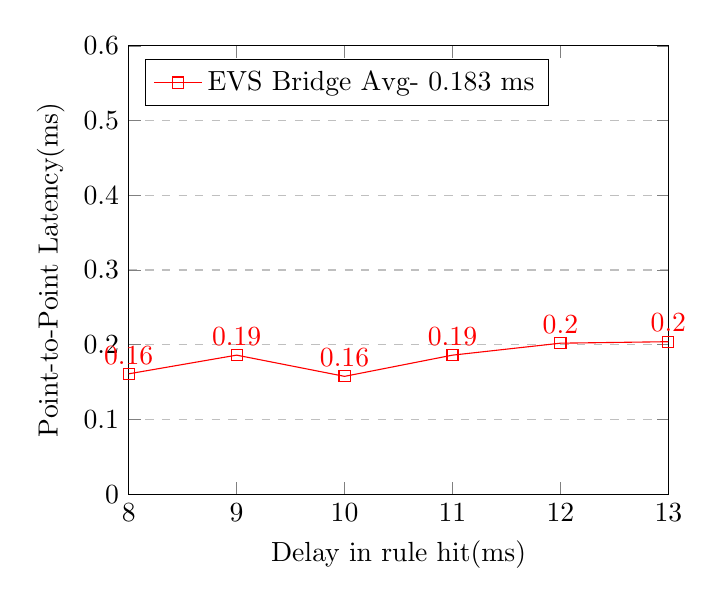
\begin{tikzpicture} 
	\begin{axis}[
	xlabel={Delay in rule hit(ms)},
	ylabel={Point-to-Point Latency(ms)},
	xtick=data,
	xmin=8, xmax=13,
	ymin=0.00, ymax=0.6,
	xtick={8,9,10,11,12,13},
	ytick={0.00,0.10,0.20,0.30,0.40,0.50,0.60},
		nodes near coords,
	legend pos=north west,
	ymajorgrids=true,
	grid style=dashed,
	]
	\addplot[
	color=red,
	mark=square,
	]
	coordinates {
		(8,0.161)(9,0.186)(10,0.1576)(11,0.186)(12,0.202)(13,0.204)
	};
	\addlegendentry{EVS Bridge Avg- 0.183 ms}
	\end{axis}
	\end{tikzpicture}
\end{figure}

Analysing the plots at Figure 5.13,5.12 and 5.11 with different maximum idle time and disabled megaflows, it is concluded that the best combination of accuracy, point-to-point latency and support for high frequency rule hit is achieved when the max-idle time for the flows is set at 1 ms. With this configuration a 100\% accuracy with an average 0.18ms latency was observed for compare operations in the conducted trial runs when the flow rule was configured to be hit every 11ms.

%\subsection{Performance measure of stateful operations on event attributes}

\section{Evaluation with DPDK}
In this section the performance evaluation of the EVS bridge is presented with KVM guest virtual machines running the evntsrc ,evntbroker and evntsink applications. This section aims to emulate a real-world datacenter deployment with applications running in virtual machines. The EVS bridge in this section is accelerated by the Intel DPDK library, and the performance of this bridge is compared against a standard OVS bridge accelerated with DPDK. The evaluation in EVS DPDK is performed to measure the latency across two parameters:
\begin{itemize}
	\item The impact of VM-context switch on latency. 
	\item The impact of megaflow disabling in DPDK on the event actions.
\end{itemize}


\subsection{System Set Up}
In this subsection the system set-up for KVM guests bridged on EVS-DPDK via the dpdkvhostuser ports is presented. The configuration set up needed for such a system is described in detail. It is assumed that the system requirements for DPDK are met.\newline
The DPDK source code is compiled with the relevant system architecture and environment. 

\begin{lstlisting}
export DPDK_DIR= /~/dpdk-stable-16.11.2
cd $DPDK_DIR
export DPDK_TARGET=x86_64-native-linuxapp-gcc
export DPDK_BUILD=$DPDK_DIR/$DPDK_TARGET
make install T=$DPDK_TARGET DESTDIR=install
\end{lstlisting}

The EVS source code is compiled with the DPDK target directory.
	\begin{lstlisting}
	cd $EVS_DIR
	./configure --enable-coverage --enable-Werror --with-dpdk=$DPDK_BUILD && make && make install
	\end{lstlisting}

The vswitchd daemon and the ovsdb-server are started in a standard manner. After which DPDK configurations are passed on to the ovsdb-server. The first command allocates memory on the two sockets of the system which is reserved for DPDK hugepages, whereas the second command gives the control of dpdkvhostuser sockets to KVM.
\begin{lstlisting}
ovs-vsctl --no-wait set Open_vSwitch . other_config:dpdk-socket-mem="4096,4096"
ovs-vsctl --no-wait set Open_vSwitch . other_config:dpdk-extra=--vhost-owner \
libvirt-qemu:kvm --vhost-perm 0666
\end{lstlisting}

After which the EVS bridge is set up with three dpdkvhostuser ports.
\begin{lstlisting}
ovs-vsctl add-br br0 -- set bridge br0 datapath_type=netdev
ovs-vsctl add-port br0 vhost-user1 -- set Interface vhost-user1 type=dpdkvhostuser
ovs-vsctl add-port br0 vhost-user2 -- set Interface vhost-user2 type=dpdkvhostuser 
ovs-vsctl add-port br0 vhost-user3 -- set Interface vhost-user3 type=dpdkvhostuser 
\end{lstlisting}

The DPDK hugepages allocations are made by running the dpdk-setup scripts. Minimum of 1G hugepage support is required by OVS.
\begin{lstlisting}
cd $DPDK_DIR/tools
./dpdk-setup.sh
Option:20
\end{lstlisting}

Next, three guest virtual machines are created. Here set up for one machine - bridge - is shown:
\begin{lstlisting}
qemu-img create -f qcow2 /~/bridge.qcow2 20G
qemu-system-x86_64 -hda /home/advith/bridge.qcow2 -cdrom /home/advith/ubuntu-16.04.2-desktop-amd64.iso \
 -boot d -enable-kvm -m 4096
\end{lstlisting}


The three guests are brought up and attached to the dpdkvhostuser ports with appropriate memory mappings to ensure fast guest to host communication.

\begin{lstlisting}
qemu-system-x86_64 -m 4096 -hda /~/bridge.qcow2 -boot c -enable-kvm -no-reboot -net none \
-chardev socket,id=char3,path=/usr/local/var/run/openvswitch/vhost-user3 \
-netdev type=vhost-user,id=mynet3,chardev=char3,vhostforce \
-device virtio-net-pci,mac=00:00:00:00:00:03,netdev=mynet3 \
-object memory-backend-file,id=mem,size=4096M,mem-path=/dev/hugepages,share=on -numa node,memdev=mem -mem-prealloc
\end{lstlisting}

 \begin{figure}[H]
	\centering
	\caption{KVM guests on EVS/OVS DPDK}
	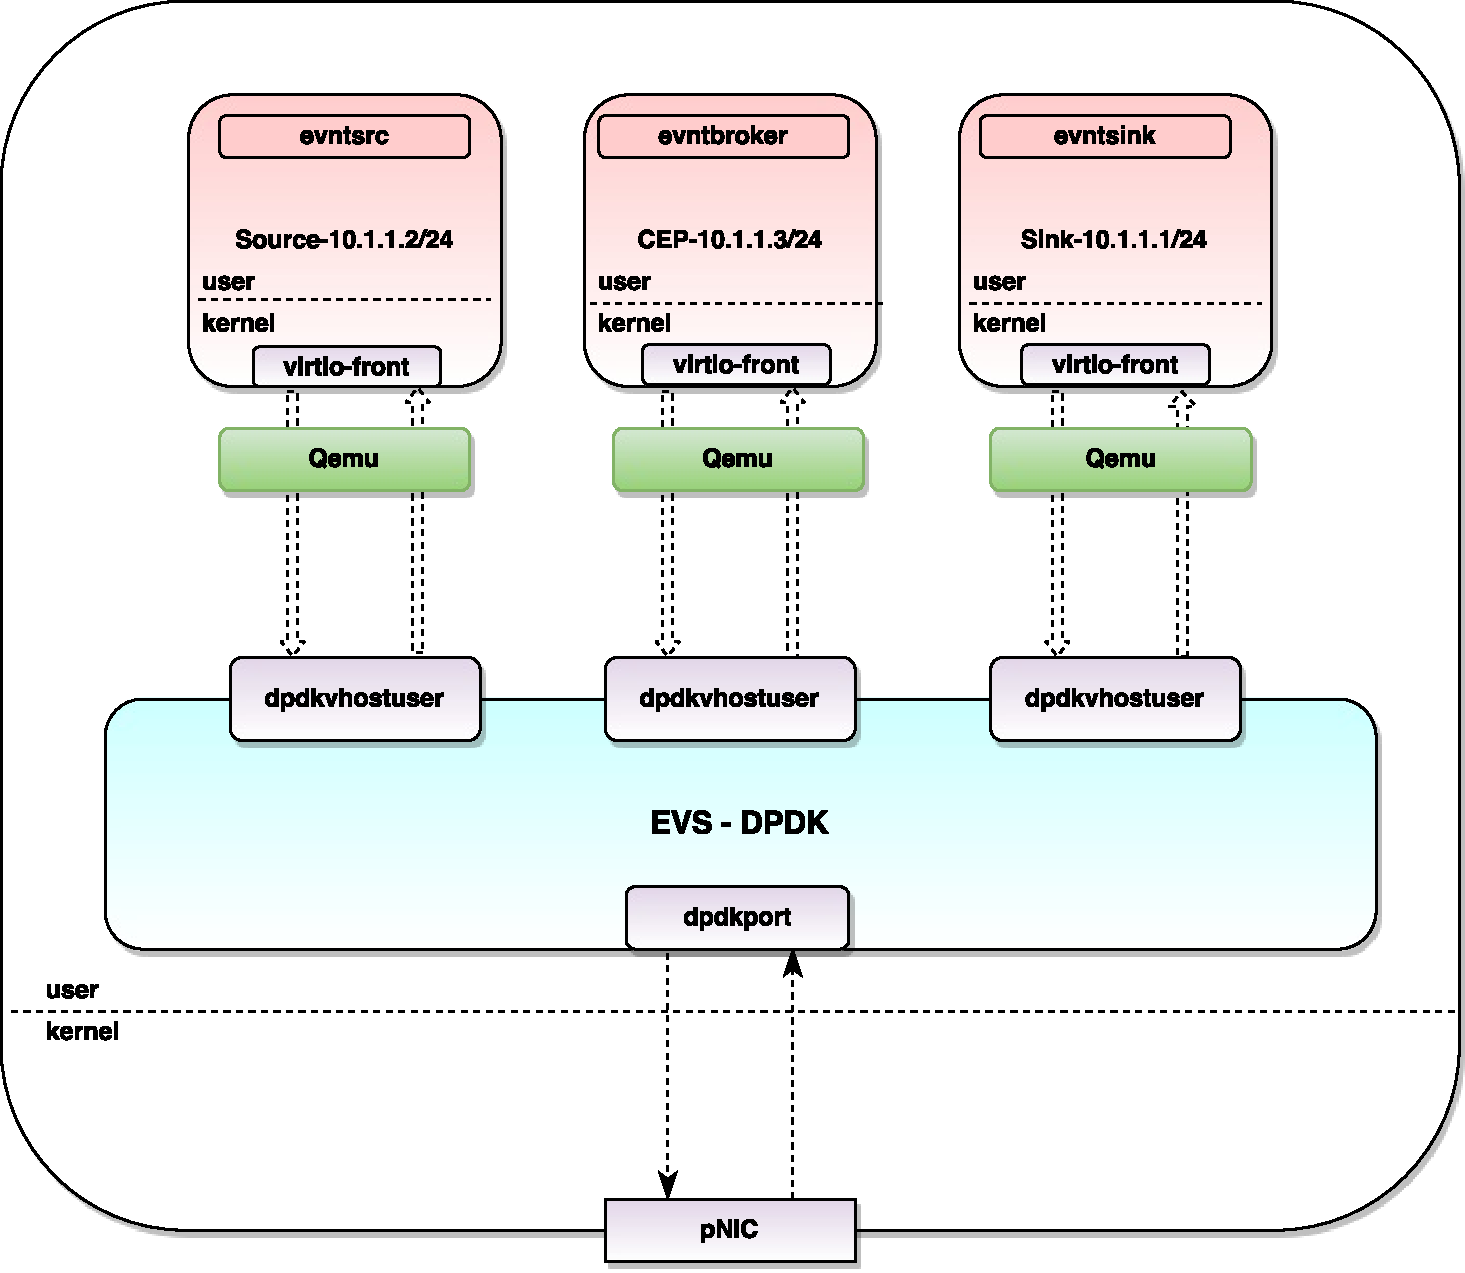
\includegraphics[height=12cm]{evsdpdk04.pdf}
\end{figure}


The set up is pictorially represented in Figure 5.14. More about the DPDK-vhost implementation is discussed in section 2.3.1. Evaluating on guest virtual machines has it's own challenges caused by clock drift. Although all the three VM's set up use the kvm_clock as the current clock source, when the system is tested with a data flow set up illustrated in Figure 5.1, the latency results are observed to be erratic. Each time the guests are restarted - which is necessary when changing from OVS to EVS - the observed latency between evntsrc and evntsink is different, sometimes even negative. This indicates that the guests clocks are drifting despite the use of kvm_clock. Although, Ubuntu specifically recommends that NTP servers shouldn't be set up within guests, the guests were set up with NTP servers to check for synchronization. However the NTP servers in guests do not solve the issue of clock drift. Given this scenario, the Evaluation on Namespaces is done by measuring the round-trip latency of the events generated by the evntsrc application. The data flow set up for the evaluation is illustrated in Figure 5.15. In case of the EVS-DPDK set up, the evntsrc application  in KVM guest-1 sends the events with a counter and a timestamp to the evntsink on KVM guest-2 via the EVS bridge. The evntsink application receives the event and retransmits with the same event to the evntsrc again via the EVS bridge. The evntsrc application on receiving the response, finds the delta between the timestamp in the event and the current timestamp to get the round-trip latency via the EVS bridge. This flow of data avoids the clock drift issue by ensuring that timestamps used to calculate the latency are generated within the same guest machine. In case of OVS, an evntbroker application on KVM guest-3 acts as the broker for events.



 \begin{figure}[H]
	\centering
	\caption{Data Flow in EVS vs OVS DPDK}
	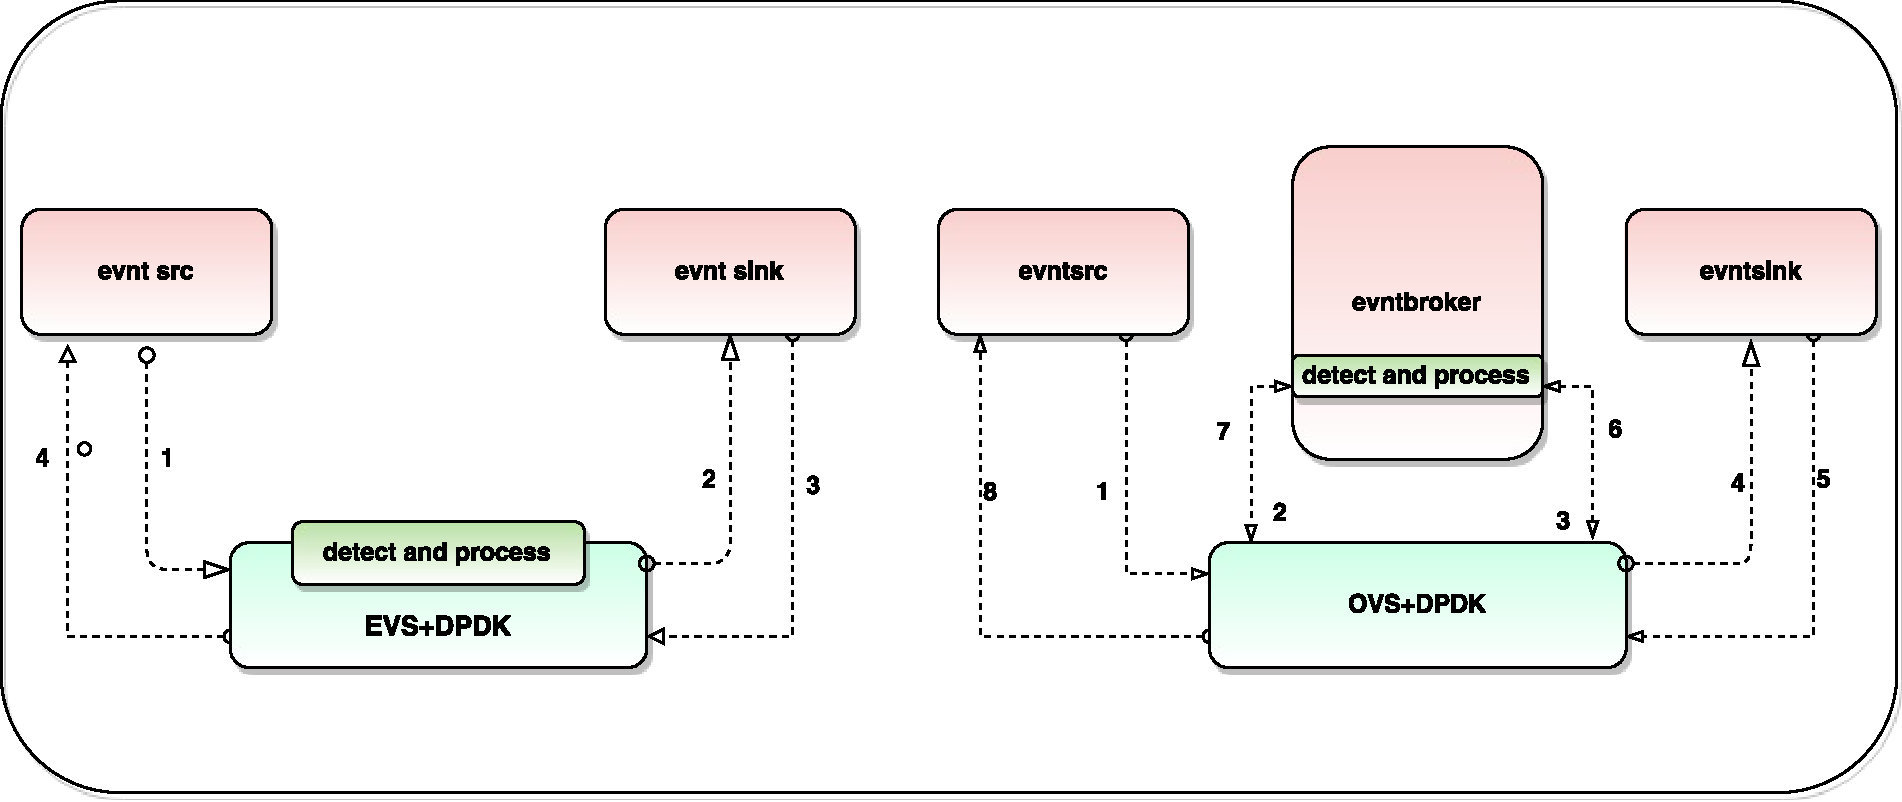
\includegraphics[height=7cm]{evsovsdpdk.pdf}
\end{figure}


The evaluation on KVM guests emulates a real-world data centre deployment. The motivation for this evaluation is to repeat the evaluation done on network namespaces, but rather find insights to the questions that are left open after evaluation on network namespaces, namely:
\begin{itemize}
	\item The impact of the additional context-switch between the hypervisor and guests on latency. 
	\item The impact of high throughput on the compare operations which in current form rely on cache re-validation. 
\end{itemize}

\subsection{Guest-to-Guest Measurements}

Having established the key questions, the initial observations on guest-to-guest communication on the EVS bridge and OVS bridge in terms of throughput, RTT and average packet processing cycles per packet are detailed in the Table 5.3. The EVS bridge introduces a three-fold increase in packet processing cycles per packet because of the additional processing needed to parse and de-serialize the events within the packet. But the burden is introduced only on tagged packets as is confirmed by the readings of per packet processing on iperf3 packets on both the bridges shown. \newline \newline



\begin{center}
	\captionof{table}{OVS vs EVS DPDK comparision} \label{tab:title} 
	\begin{tabular}{ |c|c|c| }
		\hline
		\textbf{Parameter} &  \textbf{OVS Bridg}e &  \textbf{EVS Bridge} \\\toprule
		\hline
		Throughput  & 6.40 Gbps & 6.60 Gbps  \\
		\hline 
		hping3 RTT  & 4.0 ms & 4.9 ms \\
		\hline		
		Tagged packets - Avg processing 
		cycles per packet  &  6075.91 & 20472.32  \\ 
		\hline
		\hline		
		iperf3 - Avg processing 
		cycles per packet   &  2828.63 & 2811.79 \\\bottomrule		
	\end{tabular}
\end{center} 


\subsection{Performance measurement with event detection redirection}
In this subsection, the performance evaluation of event detection and event redirection operation - 5.1 - is presented when performed on a hypervisor EVS-DPDK. This subsection is a counterpart of the evaluation performed on namespaces detailed in section 5.4.3. One key question left open by the evaluation on namespaces is whether the added context switch overhead that exists case of a hypervisor-guest deployment have an impact on the performance comparison of event detection and redirection operations performed on EVS against the same operations performed on a evntbroker in another guest. The flow of data for the evaluation is illustrated in Figure 5.15, and as described previously Round-trip latency is used instead of point-to-point latency. The event direction in case of a virtualized L2 network is done using the mod_dl_dst action unlike the mod_nw_dst action in namespaces. A similar rule is installed to handle the redirection from 10.1.1.1 to 10.1.1.3.

\begin{lstlisting}[language=json,firstnumber=1]
{
"dpid": 178974088016461,
"table_id": 0,
"priority": 11112,
"flags": 1,
"match":{
"dl_type":0x0800,
"nw_proto":17,
"nw_src":"10.1.1.2",
"nw_dst":"10.1.1.3",
"tp_dst":9877,
"e_type":"TEMP",
},
"actions":[{
"type":"set_nw_dst",
"nw_dst": 10.1.1.1
},
{
"type":"set_dl_dst",
"nw_dst": 00:00:00:00:00:01
},
{
"type":"NORMAL"
}
]
}
http://localhost:8080/stats/flowentry/add \end{lstlisting}



\begin{figure}[H]
	\centering
	\caption{Performance of event redirection in bridged virtual machines}
	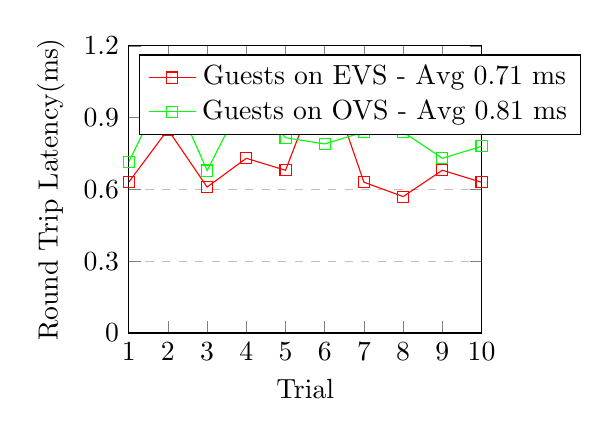
\begin{tikzpicture} [baseline=(current axis.outer east)]
	\begin{axis}[
	width=0.5\textwidth,
	xlabel={Trial},
	ylabel={Round Trip Latency(ms)},
	xmin=1, xmax=10,
	ymin=0.00, ymax=1.2,
	xtick={1,2,3,4,5,6,7,8,9,10},
	ytick={0.00,0.30,0.60,0.90,1.2},
	legend pos=north west,
	ymajorgrids=true,
	grid style=dashed,
	]
	\addplot[
	color=red,
	mark=square,
	]
	coordinates {
		(1,0.63)
		(2,0.85)
		(3,0.61)
		(4,0.73)
		(5,0.68)
		(6,1.105)
		(7,0.63)
		(8,0.57)
		(9,0.68)
		(10,0.63)
		
	};
	\addlegendentry{Guests on EVS - Avg 0.71 ms}
	\addplot[
	color=green,
	mark=square,
	]
	coordinates {
		(1,0.714)
		(2,1.05)
		(3,0.6789)
		(4,1)
		(5,0.816)
		(6,0.79)
		(7,0.84)
		(8,0.84)
		(9,0.73)
		(10,0.78)
		
	};
	\addlegendentry{Guests on OVS - Avg 0.81 ms}
	
	
	\end{axis}
	\end{tikzpicture}
\end{figure}



The results show that when event redirection is performed on EVS in a virtualization environment, removing the context switch from hypervisor to guest and back to hypervisor results in a lower round trip latency when compared to sending the events to the evntbroker for redirection. Although the improvement is marginal, this opens up avenues for exploration, especially to reduce the average processing cycle per packet.



\subsection{Testing for accuracy of compare operations}
In this subsection the accuracy of the compare operations - 5.7 and 5.8 - is evaluated in a similar fashion detailed in 5.4.9. The aim of the evaluation is to see the impact of high bandwidth on the ideal rule hit rate for compare operations. Two approaches are considered for the evaluation: 
\begin{itemize}
	\item Disabled Megaflows
	\item Max-idle time - 1 ms
\end{itemize} 




\pgfplotstableread[row sep=\\,col sep=&]{
	Delay & Disabled & Max   \\
	7     & 94.73  & 49.2   \\
	8     & 95.68 & 65.3    \\
	9    & 96.65 & 88.32 \\
	10    & 96.2 & 96.73  \\
	11    & 96.12 & 96.76  \\
}\delaydata



\begin{figure}[H]
	\noindent\hrulefill
	
	\noindent
	\caption{Accuracy of  operations in EVS DPDK}
	\begin{tikzpicture}
	\begin{axis}[
	ybar,
	xlabel={Delay in Rule hit (ms)},
	ylabel={Accuracy of compare operations(percentage)},
	symbolic x coords={7,8,9,10,11},
	nodes near coords,
	legend style={at={(0.5,1)},
		anchor=south,legend columns=-1},
	]
	\addplot[fill=green] table[x=Delay,y=Disabled]{\delaydata};
	\legend{Disabled Megaflow}
	\end{axis}
	\end{tikzpicture}
	\hfil
	\begin{tikzpicture}
	\begin{axis}[
	ybar,
	xlabel={Delay in Rule hit (ms)},
	ylabel={Accuracy of compare operations(percentage)},
	symbolic x coords={7,8,9,10,11},
	nodes near coords,
	legend style={at={(0.5,1)},
		anchor=south,legend columns=-1},
	]
	\addplot[fill=red ] table[x=Delay,y=Max]{\delaydata};
	\legend{Max Idle Time 1ms}
	\end{axis}
	\end{tikzpicture}
\end{figure}


As plotted in the graph in figure 5.17, with disabled megaflows the EVS supports an accuracy of 94\% to 97\% when a flow rule is hit every 7ms, whereas with a configure idle time of 1 ms, an accuracy of 96\% is acheived only at a rule hit rate of 10 ms. This can be contrasted with the results in figure 5.11 and 5.12 where higher levels of accuracy were hit. To understand this difference more work is done on the cache revalidation process in Open vSwitch. A future work may involve changing the re-validator to evict event processing rules at a higher rate compare to the other OpenFlow rules.


\subsection{Evaluation of processing cycles needed for event operations}
 The event processing pipeline in EVS is expensive in general, as show in table 5.3. Each tagged packet in this pipeline averages three times the average processing cycle. In this subsection, the evaluation of processing cycles needed  for event operations is presented.
 
 
\begin{center}
	\captionof{table}{Processing cycles for event operations} \label{tab:title} 
	\begin{tabular}{ |c|c| }
		\hline
		\textbf{Parameter} &  \textbf{Average processing cycles per packet} \\\toprule
		\hline
		Tagged packets without detection  &  20472.9 \\
		\hline 
		Tagged packets with event type detection  & 20039.28 \\
		\hline		
		Tagged packets with event type and one attribute detection  &  20322.76  \\ 
		\hline
		Tagged packets with event type and two attributes detection  &  18623.9  \\ 
		\hline		
		Tagged packets with compare operations with disabled megaflow    &  83275.34  \\\bottomrule		
	\end{tabular}
\end{center} 

The processing cycles need per packet does not seem to vary as detection operations are performed on event attributes. However, when compare operations are performed with disbled megaflows, as they should be to reach an acceptable level of accuracy, the number of processing cycles needed nearly quadruple. This is because of the cache miss and additional Openflow pipeline look up per packet also observed indirectly as the increased point to point latency for these operations in figure 5.11 and 5.12.


